\section{The Desktop Application}\label{sec:app}

\begin{figure*}[t]
\centering
\begin{tikzpicture}
\node[inner sep=0, draw=black!35] (a) {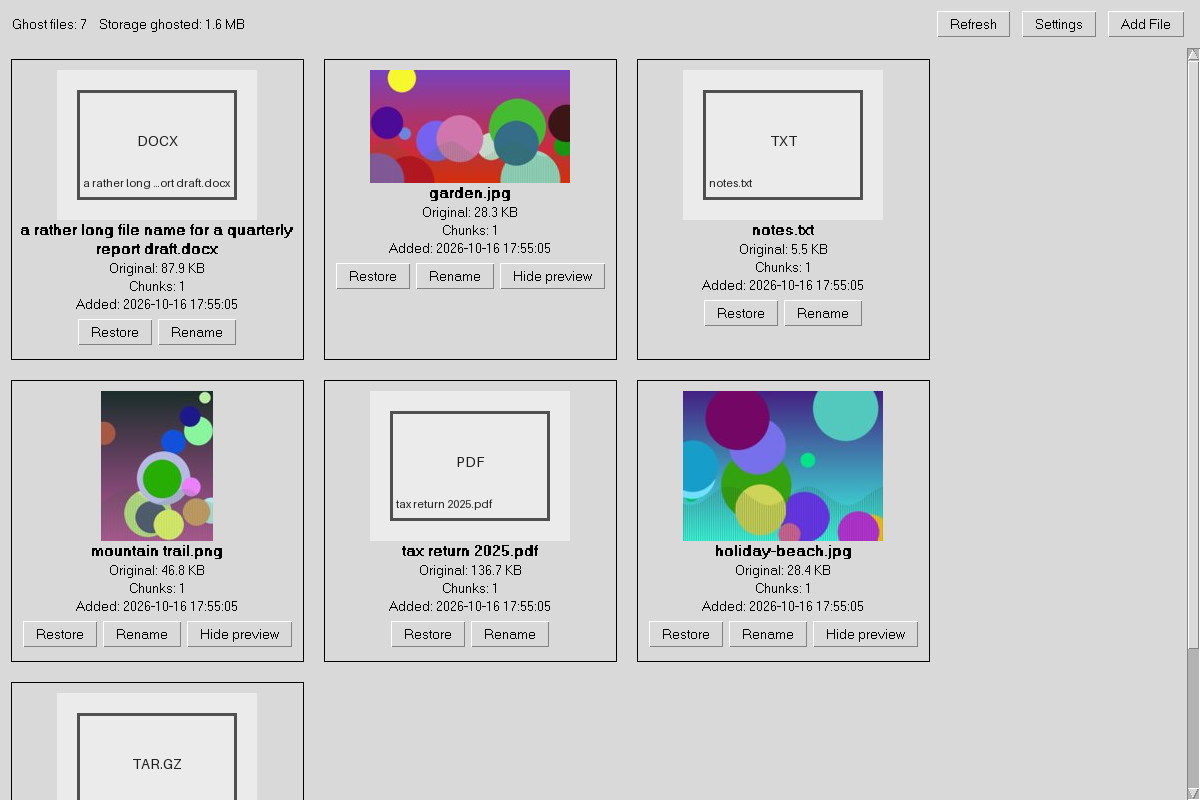
\includegraphics[width=86mm]{images/main-window.png}};
\node[inner sep=0, draw=black!35, right=5mm of a] (b) {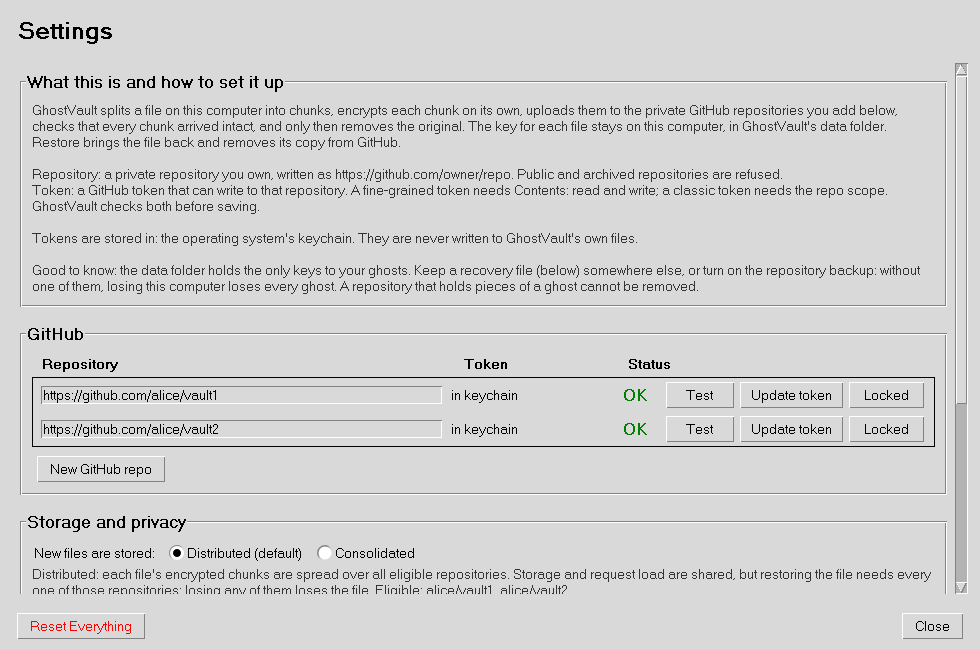
\includegraphics[width=86mm]{images/settings.png}};
\node[font=\footnotesize, below=1.5mm of a] {(a) the main window: one card per ghost};
\node[font=\footnotesize, below=1.5mm of b] {(b) Settings: repositories, storage and privacy, recovery};
\end{tikzpicture}
\caption{The interface, captured against the simulated GitHub with generated sample files. Image
ghosts show their decrypted preview; other files a placeholder drawn in memory. The captures were
made under Xvfb with Tk's X11 core fonts; a desktop with anti-aliased fonts draws the same layout with
smoother text.}
\label{fig:screens}
\end{figure*}

\subsection{The window}
The interface is built from Tk's classic widgets (\figref{fig:screens}). The main window has a bar
with the statistics and three buttons, a progress area that appears while an operation runs, and a
gallery of cards. Settings is a second window with sections for the repositories and their tokens,
storage and privacy (placement, eligible repositories, padding, previews), and recovery. Text worth
copying, such as names, paths, messages and recovery details, can be selected and copied, and every
action can be reached from the keyboard. Every size given in pixels is multiplied by the display's
scale, so the layout keeps its proportions at 125, 150 or 200\,\%; on Windows the process declares
itself DPI-aware so that text is sharp.

\subsection{Work off the window's thread}
Ghosting, restoring, every other operation and every network request run off the window's thread.
An operation that changes the vault runs on a worker thread, one at a time, while the window shows its progress and its
percentage in the title. Small read-only work runs on a pool of two threads: reading a repository's
backup status, and decrypting and decoding previews, except that cached previews are decrypted on the
window's thread for up to 60\,ms per refresh, so that the gallery appears at once. Workers hand their results back through queues that the window thread polls every
60\,ms, and only the window thread touches Tk. If the user closes the window during an operation and
confirms, the process ends at once with the data folder still locked, and the next start finishes or
undoes the operation from its journal, exactly as after a crash; letting the worker continue after
the lock was released could let a second GhostVault act on the same records.

\subsection{Secrets in the interface}
Recovery keys and generated passphrases are shown once, hidden until the user presses \emph{Show},
and copied only by an explicit Copy. A copied secret is taken off the clipboard after one minute and
when GhostVault closes, but only if the clipboard still holds exactly that secret, so anything copied
since is left alone. GhostVault cannot remove copies kept by a clipboard history or a synchronised
clipboard, and the dialog says so. Passphrase and token fields are masked.

\subsection{The log}
The log, \code{logs/ghostvault.log}, is owner-only and rotates at 1\,MB, keeping three old files. It
names ghosts by their ids and repositories by name; it never records the names of the user's files,
keys or tokens. Exceptions are logged by type and place only (file name, line and function of the
innermost frames), never with their message, which can hold a path or a secret; the log's formatter
applies the same rule to any traceback, so no later code can write one in full by mistake.

\subsection{Standalone applications}\label{sec:builds}
Releases contain standalone applications for Windows (x86-64), macOS on Apple silicon and on
Intel, and Linux (x86-64), alongside the Python package (\tabref{tab:release}). Each is a one-folder
PyInstaller~\cite{pyinstaller} build containing Python 3.13, Tcl/Tk and GhostVault's dependencies;
it uses the same data folder as the Python package. One script, \code{packaging/build.py}, builds
locally and in the release workflow, in four steps:
\begin{enumerate}
\item \emph{freeze}: PyInstaller, then license notices generated from the bundled distributions'
metadata, Python's and Tcl/Tk's licenses and, on Linux, the copyright files of the system packages
whose libraries were bundled; then the signature, where configured;
\item \emph{smoke}: the application is started with \code{--version} and \code{--self-check}, which
checks the encryption library, the image decoders, the operating system's certificate store, the
keychain backend and Tk; then its window must open and run for five seconds without logging an
error;
\item \emph{package}: the installer and portable archive, disk image or tar archive;
\item \emph{verify}: the package is unpacked, mounted or installed, and the application in it is
checked again. The Windows installer installs into a scratch folder and uninstalls; on Linux,
\code{install.sh}, an update over it and \code{uninstall.sh} run in a scratch home folder, and the
data folder must come through untouched.
\end{enumerate}
The minimum system of each build is computed from its binaries (the macOS version from the Mach-O
load commands, the glibc version from the ELF symbol versions) and stated in the release notes.

\begin{table}[t]
\caption{Files of a release}\label{tab:release}
\centering\footnotesize
\begin{tabular}{@{}L{29mm}L{51mm}@{}}
\toprule
\textbf{System} & \textbf{File} \\
\midrule
Windows 10 and 11, x64 & installer (Inno Setup; per user by default, without administrator rights)
and portable zip; a windowed \code{GhostVault.exe} and a console \code{ghostvault-cli.exe} \\ \addlinespace[1.6pt]
macOS, Apple silicon & disk image with \code{GhostVault.app} \\ \addlinespace[1.6pt]
macOS, Intel & disk image with \code{GhostVault.app} \\ \addlinespace[1.6pt]
Linux, x86-64 & tar archive with \code{install.sh} and \code{uninstall.sh} (per user, with a menu
entry) \\ \addlinespace[1.6pt]
any, Python 3.11+ & wheel and source distribution \\ \addlinespace[1.6pt]
all & \code{SHA256SUMS.txt} \\
\bottomrule
\end{tabular}
\end{table}

Signing is optional and configured through repository secrets. Without them, the Windows files are
unsigned, the macOS applications carry an ad-hoc signature, and the release notes say so; users can
check every file against \code{SHA256SUMS.txt}. With a certificate, Windows files are signed with
\code{signtool} (SHA-256, timestamped); a signing command can replace the certificate file for keys
held in hardware or a signing service. On macOS, PyInstaller signs every binary with a Developer ID,
the hardened runtime and a secure timestamp; with a notarization key, the application and then the
disk image are notarized and stapled.

The release workflow (\code{.github/workflows/release.yml}) runs the complete CI checks, then builds
and verifies on four GitHub-hosted runners (\path{windows-2025}, \path{macos-15}, \path{macos-15-intel},
\path{ubuntu-22.04}),
collects the Python package, checksums and release notes, and, for a version tag only, creates a
\emph{draft} release; it is the only job with permission to write to the repository, and it refuses
to change a release that has been published. The workflow needs no secrets or settings, so it runs
as it is in any repository, including a separate build repository. The status of these builds is
in \secref{sec:status}.
